\documentclass[a4paper,12pt]{article}
\usepackage{fullpage}  % leaves 1 inch margins all round
\usepackage{iftex}
\ifPDFTeX
  \usepackage[T1]{fontenc} % modern encoding (more characters available)
  \usepackage{mathptmx} % times in text and mathematics
  \usepackage[scaled]{helvet} % helvetica for sanserif, scaled 95% by default
  \usepackage{courier}  % for typewriter text
\else
  \usepackage{fontspec}
  \usepackage{unicode-math}
  \setmainfont{Times New Roman}
  \setsansfont{Arial}
  \setmonofont{Consolas}
  \setmathfont{Cambria Math}
\fi
\usepackage{textcomp} % lots of useful symbols
\usepackage{graphicx}  % inclusion of graphics files
\usepackage{amsmath}
\usepackage{cite}


\begin{document}

\title{How to write a technical project report}
\author{School of Engineering, University of Glasgow}
\date{\today}
 
\maketitle

\begin{abstract}
All reports start with an \emph{abstract}, which contains a summary of the project: its aim, what was done and what was achieved. This document describes the requirements for a project report in the department and gives advice on how to get better marks. It is structured to match a project report as far as possible.
\end{abstract}

%\tableofcontents

\section{Introduction}

\emph{Whew -- I've finished the work, now I only have to write the report.} Sound familar? Many students put off writing until too late and don't leave enough time to make a good job of the report. This is a serious mistake because the report typically accounts for a large fraction of the assessment. Start early -- most people find report-writing difficult. Think about the report throughout your project, keep track of references and collect material to illustrate the report.

\subsection{Mechanical aspects}

The length of the body of the report will be specified in the instructions for the project. Extra material may be provided in appendices but this material should be for reference only: you cannot assume that the reader will study it. In other words, do not put vital points in an appendix.

You will probably think that the report is too short but this is deliberate. Most reports are submitted to busy managers, who do not have time to read lengthy documents. It is important to learn how to pick out the vital points and write a concise report with maximum impact.

Reports should be word-processed and firmly bound. Use A4 paper and a clear typeface such as 12-point Times, number the pages and leave margins of at least 25\,mm all round. Follow this layout (this document breaks some of the rules to keep it compact).
\begin{itemize}
\item
The front cover should show the title of the project with your name(s) and matriculation number(s) and the name of your supervisor(s).
\item
Put the abstract on the next page. It should be about 100--250 words and gives a brief summary of the report including the background and aims of the project, the principal results and conclusions.
\item
The next page should show the table of contents. 
\item
The body of the report should be divided into numbered sections, each starting on a new page. Figures (diagrams, plots or photographs) and tables need captions and should be numbered.
\end{itemize}

\subsection{What goes into the introduction?}

Explain the background to the project and the reasons why your particular piece of work was considered worthwhile. This leads to the \textbf{aims} of the project: what you are trying to achieve. Be specific.


\section{Body of the report}

\subsection{Experimental protocol and basic settings}

This work was carried out in two phases. The first phase contains the early exploratory experiments, which were used to establish an initial baseline and to see whether input enhancement or loss design changed segmentation behaviour in a meaningful way. The second phase contains the main experiments on the DRIVE dataset \cite{staal2004drive}, where the proposed structural modifications were evaluated under a unified five-fold cross-validation protocol. Because these two phases differ in data source, input format, split strategy, and evaluation metrics, they are described separately.

The early phase covers Experiments 1--3. These runs used multi-source training data to build the first version of the model and to test simple changes in preprocessing and loss design. The later phase starts from Experiment 4, which defined the common DRIVE baseline. Experiment 5 and every structural variant after that used the same dataset, preprocessing pipeline, and five-fold split, so their differences can be compared directly.

\subsubsection{Datasets and data organization}

During the early exploratory phase, the training data came from several public retinal vessel segmentation datasets, including STARE \cite{hoover2000locating}, CHASE\_DB1 \cite{fraz2012ensemble}, and HRF \cite{budai2013robust}. Rather than creating a new split, Experiments 1--3 reused the existing training and validation lists from the senior student's setup. That kept the setting directly comparable to the earlier work. Under this split, the training and validation sets contained 801 and 90 samples, respectively.

For input construction in the early phase, each color fundus image was converted into the NIfTI format required by nnU-Net and then separated into red, green, and blue channels, which were fed to the model individually. This preserved the original spectral information and made it possible to inspect what each channel contributed. It also set up the later discussion of green-channel cues and contrast enhancement.

The later experiments used DRIVE only and followed one data pipeline throughout. Instead of three-channel color input, each image was converted to grayscale, normalized, processed with contrast-limited adaptive histogram equalization, adjusted by gamma correction, and saved as a single-channel NIfTI file. This preprocessing matches the setting in PA-Net \cite{luo2025panet}. In practice, it made thin vessels and low-contrast regions easier to see while removing color information that was not especially useful for the task.

From Experiment 4 onward, the data organization and five-fold split remained fixed. That is why the later performance differences are attributed mainly to changes in network structure, loss design, or post-processing rather than to changes in the data split.

\subsubsection{Implementation details and evaluation metrics}

All experiments were implemented within the nnU-Net v2 framework \cite{isensee2021nnunet}. Within each phase, the training workflow was kept fixed unless a change was part of the experiment itself. In practice, the later experiments mainly modified the U-Net backbone inside nnU-Net and the way features interacted across stages; only a few runs changed the loss setting or trainer-level strategy. The early phase used a fixed split to test feasibility, whereas the later phase used the 2D nnU-Net configuration on DRIVE with five-fold cross-validation to evaluate the structural changes.

In the early phase, the baseline model used the standard nnU-Net trainer and ran for 150 epochs. Experiments 1--3 correspond to the raw-input baseline, the CLAHE-enhanced input, and the CLAHE version trained with Dice loss plus Focal Loss. The evaluation script reported IoU for the vessel class, mIoU, Recall, Precision, Accuracy, mPA, and F1-score, and the early results are presented with that metric set.

In the later phase, all models used the 2D nnU-Net v2 configuration with a \(512 \times 512\) input patch size, batch size 2, and 100 training epochs. Optimization used SGD with an initial learning rate of 0.001 and a Poly schedule. Unless noted otherwise, every model shared the same split and training plan. Experiment 4 served as the baseline for this phase, and Experiment 5 plus all later variants were compared under that common setting.

For evaluation, the later phase used the aggregated outputs from all five folds rather than the result of any single fold. Each fold contributed predictions for its validation subset, and the final metrics were computed on the combined cross-validation output. This avoids leaning too heavily on one split and makes comparisons more stable.

The later phase reports Sensitivity (SE), Specificity (SP), Accuracy (ACC), AUC, Precision (PR), and F1-score. SE reflects how well the model captures thin vessels and weak responses. SP and PR indicate how well it controls false positives. ACC measures overall pixel accuracy, and F1-score summarizes overall segmentation quality. Because probability maps were not saved in the current experiments, AUC was approximated from binary predictions.

\subsection{Baseline and early explorations}

The first three experiments were used as an early checkpoint before moving to structural changes. They reused the existing training and validation lists so the results stayed directly comparable with the senior student's setup. All three used DRIVE for testing and were evaluated with the same early-stage metrics.

Experiment 1 used the standard nnU-Net baseline \cite{isensee2021nnunet}. It produced stable overall segmentation under the fixed split and gave a practical reference point for the rest of the study.

Experiment 2 added CLAHE under the same training setup. Training stabilized earlier, but the final segmentation metrics did not improve much. In other words, clearer input alone was not enough to solve the harder cases, especially thin vessels and complex branching regions.

Experiment 3 kept the CLAHE input and added Focal Loss to put more emphasis on hard pixels and class imbalance. Convergence became even faster, but the performance gain still did not hold up at the end. That points to the same conclusion: with the current network, changing the loss alone was not enough to move the baseline in a reliable way.

Viewed together, these experiments helped narrow the problem. Input enhancement and loss design changed optimization behaviour, but they did not really change how the model represented thin vessels, low-contrast areas, or structural continuity. That is why the later work shifted from training-level tweaks to structural changes.

\begin{table}[htbp]
\centering
\caption{Summary of early exploratory experiments}
\label{tab:early_experiments_en}
\begin{tabular}{llllll}
\hline
Experiment & Method & Training setting & Convergence & Representative result & Main observation \\
\hline
Exp1 & nnU-Net baseline & Dice, 150 epoch & Converged at epoch 69 & F1 = 0.7924 & Established the early baseline \\
Exp2 & CLAHE + nnU-Net & Dice, 150 epoch & Converged at epoch 60 & F1 = 0.7827 & Faster early convergence, limited final gain \\
Exp3 & CLAHE + nnU-Net + Focal Loss & Focal Loss, 150 epoch & Converged at epoch 53 & F1 = 0.7802 & Faster convergence, no further performance gain \\
\hline
\end{tabular}
\end{table}

\subsection{PA-Net module migration}

After the baseline and early explorations, the next step was to bring two PA-Net modules into nnU-Net: the Lightweight Parallel Transformer (LPT) and the Adaptive Vascular Feature Fusion Module (AFFM) \cite{luo2025panet}. This was not meant as a final model. It was a way to see whether PA-Net's main design ideas were useful in the current setting and, if so, which parts were worth keeping.

LPT was placed at the bottleneck to improve long-range dependency modeling and the representation of global vessel structure. In PA-Net, LPT combines local feature processing with parallel attention at relatively low computational cost. For retinal vessel segmentation, that could help the model keep a more complete picture of vessel layout in high-level features, especially where thin vessels tend to break or disappear. AFFM replaced the standard skip-fusion step and let features from different levels interact through adaptive weighting instead of direct concatenation. That gave shallow detail and deep semantic cues different roles during decoding. In this task, the hoped-for benefit was better recovery of boundaries and branching regions with less detail loss after downsampling.

In an abstract form, if the input feature is denoted by \(X\), the attention branch in LPT can be written as
\[
Q = XW_Q,\qquad K = XW_K,\qquad V = XW_V,
\]
\[
\mathcal{A}(X) = \mathrm{Softmax}\left(\frac{QK^{\top}}{\sqrt{d}}\right)V,
\]
where \(d\) denotes the feature dimension. If the local branch is further denoted by \(\mathcal{L}(X)\), the LPT output can be summarized as
\[
Y_{\mathrm{LPT}} = \mathrm{FFN}\big(\mathcal{L}(X) + \mathcal{A}(X)\big) + X.
\]
This form shows that the key role of LPT is not merely to introduce attention, but to combine local feature extraction and global dependency modeling in parallel before fusion. For AFFM, if the three input features from different levels are denoted by \(F_1\), \(F_2\), and \(F_3\), its fusion process can be simplified as
\[
Y_{\mathrm{AFFM}} = \sum_{i=1}^{3}\alpha_i \odot F_i,\qquad
[\alpha_1,\alpha_2,\alpha_3] = \mathrm{Softmax}\big(\phi([F_1,F_2,F_3])\big),
\]
where \(\phi(\cdot)\) denotes the weight generation function implemented by convolution, and \(\odot\) denotes element-wise weighting. In other words, AFFM lets the decoder reweight information from different levels instead of treating them equally.

\begin{figure}[htbp]
\centering
\begin{minipage}{0.45\textwidth}
\centering
\includegraphics[height=0.22\textheight,keepaspectratio]{pic/panet.png}\\
(a) Overall PA-Net architecture
\end{minipage}
\hfill
\begin{minipage}{0.2\textwidth}
\centering
\includegraphics[height=0.22\textheight,keepaspectratio]{pic/LPT.png}\\
(b) Structure of the LPT module
\end{minipage}
\hfill
\begin{minipage}{0.33\textwidth}
\centering
\includegraphics[height=0.22\textheight,keepaspectratio]{pic/AFFM.png}\\
(c) Structure of the AFFM module
\end{minipage}
\caption{PA-Net and the two core modules migrated into nnU-Net. All three images use the same height for direct visual comparison.}
\label{fig:panet_triplet_en}
\end{figure}

LPT and AFFM were first added together and compared with the baseline under the unified protocol. That gave a direct view of what full PA-Net-style migration looked like inside nnU-Net and set up the ablation work that followed. Since the later experiments mostly modified the U-Net backbone and feature interactions, this combined version served as the starting point for the next round of analysis. The next section therefore looks at LPT and AFFM separately.

\subsection{Ablation of LPT and AFFM}

Once the full PA-Net-style migration was in place, the obvious next question was which module was actually driving the change in performance. To answer that, this section kept the later-stage protocol fixed: the same single-channel preprocessing, the same five-fold split, and the same training schedule on DRIVE. As before, the metrics were computed after combining the validation outputs from all five folds.

Because nnU-Net is tightly coupled to its backbone, the comparison included three models beyond the baseline: the full PA-Net migration, LPT Only, and AFFM Only. LPT Only corresponds to Ablation A and adds LPT at the bottleneck only. AFFM Only corresponds to Ablation B and changes only the decoder-side feature fusion.

\begin{table}[htbp]
\centering
\caption{Comparison of LPT and AFFM ablation results}
\label{tab:lpt_affm_ablation_en}
\resizebox{\textwidth}{!}{
\begin{tabular}{lcccccc}
\hline
Experimental group & SE & SP & ACC & AUC & PR & F1-score \\
\hline
nnU-Net v2 Baseline & $0.7627 \pm 0.0446$ & $0.9852 \pm 0.0050$ & $0.9659 \pm 0.0045$ & $0.8739 \pm 0.0210$ & $0.8238 \pm 0.0646$ & $0.7891 \pm 0.0320$ \\
PA-Net (Full) & $0.7211 \pm 0.0763$ & $0.9888 \pm 0.0050$ & $0.9659 \pm 0.0059$ & $0.8549 \pm 0.0365$ & $0.8570 \pm 0.0621$ & $0.7782 \pm 0.0464$ \\
LPT Only (Ablation A) & $0.7597 \pm 0.0492$ & $0.9864 \pm 0.0041$ & $0.9669 \pm 0.0044$ & $0.8731 \pm 0.0234$ & $0.8361 \pm 0.0546$ & $0.7935 \pm 0.0297$ \\
AFFM Only (Ablation B) & $0.7573 \pm 0.0475$ & $0.9868 \pm 0.0039$ & $0.9672 \pm 0.0045$ & $0.8720 \pm 0.0227$ & $0.8400 \pm 0.0517$ & $0.7942 \pm 0.0300$ \\
\hline
\end{tabular}
}
\end{table}

Table \ref{tab:lpt_affm_ablation_en} shows a fairly clear pattern. The full PA-Net migration did not outperform the baseline, while the two single-module variants behaved more steadily. LPT Only kept SE almost unchanged and slightly improved PR and F1-score, which makes LPT a reasonable direction to keep exploring. AFFM Only reached the highest ACC and F1-score within this small comparison, but the margin was limited and not strong enough to make AFFM the main focus of the later experiments.

The takeaway from this section is modest but useful. Individual ideas from PA-Net were still worth examining, but moving LPT and AFFM into nnU-Net as a bundle did not produce a better overall structure. The main value of this experiment was to narrow down where the drop might be coming from, not to declare a final direction. That is why the next steps looked more closely at the modules themselves and at how they interacted with the existing training setup. More detailed metric-level discussion is left to Chapter 3.

\subsection{Compatibility check between AFFM and deep supervision}

AFFM in PA-Net is used for multi-level decoder fusion \cite{luo2025panet}, while deep supervision in nnU-Net also acts on multi-scale decoder features \cite{isensee2021nnunet,lee2015dsn}. Since the two mechanisms affect similar parts of the network, an extra control experiment was added to check whether they conflicted in the current framework. The same later-stage protocol was used again: single-channel preprocessing, the same five-fold split, and the same DRIVE training schedule. Metrics were still computed after aggregating all five folds.

In the default nnU-Net training procedure, deep supervision applies auxiliary segmentation losses at multiple decoder stages in order to strengthen multi-scale feature learning \cite{isensee2021nnunet,lee2015dsn}. If the loss of the main output is denoted by \(\mathcal{L}_{\mathrm{main}}\) and the loss of the \(s\)-th auxiliary output is denoted by \(\mathcal{L}_{\mathrm{aux}}^{(s)}\), the total loss can be written as
\[
\mathcal{L} = \mathcal{L}_{\mathrm{main}} + \sum_{s=1}^{S}\lambda_s \mathcal{L}_{\mathrm{aux}}^{(s)},
\]
where \(\lambda_s\) denotes the weight of each auxiliary branch. Fig. \ref{fig:deep_supervision_en} shows the setup: auxiliary heads are attached to several decoder stages during training, but only the main output is used at inference. To test whether AFFM was interacting poorly with this mechanism, deep supervision was turned off in AFFM Only, creating an AFFM w/o DS model. Table \ref{tab:affm_ds_en} compares the two settings.

\begin{figure}[htbp]
\centering
\includegraphics[width=0.95\textwidth]{pic/deep_supervision.png}
\caption{Illustration of the deep supervision mechanism in the nnU-Net decoder. During training, auxiliary segmentation heads are attached to multiple decoder stages and contribute to the weighted total loss, whereas only the main output is retained during inference.}
\label{fig:deep_supervision_en}
\end{figure}

\begin{table}[htbp]
\centering
\caption{Comparison of AFFM results with and without deep supervision}
\label{tab:affm_ds_en}
\resizebox{\textwidth}{!}{
\begin{tabular}{lcccccc}
\hline
Experimental group & SE & SP & ACC & AUC & PR & F1-score \\
\hline
AFFM Only (with DS) & $0.7573 \pm 0.0475$ & $0.9868 \pm 0.0039$ & $0.9672 \pm 0.0045$ & $0.8720 \pm 0.0227$ & $0.8400 \pm 0.0517$ & $0.7942 \pm 0.0300$ \\
AFFM w/o DS & $0.7401 \pm 0.0493$ & $0.9880 \pm 0.0038$ & $0.9667 \pm 0.0048$ & $0.8640 \pm 0.0236$ & $0.8490 \pm 0.0534$ & $0.7883 \pm 0.0308$ \\
\hline
\end{tabular}
}
\end{table}

The result is fairly straightforward. Turning off deep supervision slightly increased SP and PR, but SE, AUC, and F1-score all went down. The model became more conservative: it produced fewer false positives, but it also missed more thin vessels and weak responses.

So removing deep supervision did not rescue the AFFM-based model. At most, it explains part of the precision change, not the overall behaviour seen earlier. The point of this experiment was mainly to rule out one possible source of the problem and to show that AFFM did not yield a stable gain in the current framework. Whether AFFM should stay in the design was left open until the later structural experiments. Chapter 3 revisits this in more detail.

\subsection{Deformable attention in LPT}

After the control experiment on AFFM and deep supervision, attention shifted back to LPT itself. The goal here was to see whether its high-level feature modeling could be improved by replacing the original GAA operation in PA-Net LPT \cite{luo2025panet} with deformable attention \cite{zhu2021deformabledetr}. This replacement was motivated by the shape of retinal vessels: curved segments, bifurcations, and thin peripheral branches are hard to capture with rigid sampling patterns. The experiments again used the same later-stage protocol on DRIVE, with metrics computed from the aggregated outputs of all five folds.

Unlike the more regular fixed sampling pattern in GAA, deformable attention learns a set of offsets for each reference position, so that feature aggregation can be distributed more flexibly around the target structure. If the reference position is denoted by \(p\), the \(k\)-th sampling offset by \(\Delta p_k\), and the corresponding weight by \(A_k\), the local aggregation can be written as
\[
\mathrm{DefAttn}(p) = \sum_{k=1}^{K} A_k \cdot x(p + \Delta p_k),\qquad
\sum_{k=1}^{K} A_k = 1,
\]
where \(K\) denotes the number of sampling points. For retinal vessel segmentation, this means sampling no longer has to follow fixed directions; it can move toward curved vessels, bifurcations, and thin peripheral branches more naturally. Fig. \ref{fig:deformable_attention_en} illustrates the difference between the GAA sampling pattern and deformable attention. Here, 4 point and 8 point simply refer to the number of sampling points around each reference position.

\begin{figure}[htbp]
\centering
\includegraphics[width=0.95\textwidth]{pic/Deformable_Attention.png}
\caption{Illustration of the sampling difference between GAA and deformable attention. The left panel shows a more regular fixed sampling pattern, while the right panel shows adaptive offset-based sampling around the reference position.}
\label{fig:deformable_attention_en}
\end{figure}

The first model in this section was Deformable LPT without AFFM (4 point), which isolated the effect of the attention replacement itself. AFFM was then added back under the same setting to see whether it still helped once LPT had changed. Finally, the sampling pattern was expanded from 4 point to 8 point to test whether a larger sampling set was useful. Table \ref{tab:deformable_lpt_en} lists the results.

\begin{table}[htbp]
\centering
\caption{Comparison of experiments related to deformable LPT}
\label{tab:deformable_lpt_en}
\resizebox{\textwidth}{!}{
\begin{tabular}{lcccccc}
\hline
Experimental group & SE & SP & ACC & AUC & PR & F1-score \\
\hline
LPT Only & $0.7597 \pm 0.0492$ & $0.9864 \pm 0.0041$ & $0.9669 \pm 0.0044$ & $0.8731 \pm 0.0234$ & $0.8361 \pm 0.0546$ & $0.7935 \pm 0.0297$ \\
Deformable LPT (No AFFM, 4 point) & $0.7634 \pm 0.0540$ & $0.9863 \pm 0.0043$ & $0.9672 \pm 0.0044$ & $0.8749 \pm 0.0254$ & $0.8371 \pm 0.0511$ & $0.7958 \pm 0.0275$ \\
Deformable LPT + AFFM & $0.7571 \pm 0.0495$ & $0.9867 \pm 0.0042$ & $0.9670 \pm 0.0044$ & $0.8719 \pm 0.0235$ & $0.8388 \pm 0.0545$ & $0.7933 \pm 0.0301$ \\
Deformable LPT (No AFFM, 8 point) & $0.7573 \pm 0.0506$ & $0.9869 \pm 0.0038$ & $0.9672 \pm 0.0047$ & $0.8721 \pm 0.0241$ & $0.8412 \pm 0.0504$ & $0.7946 \pm 0.0296$ \\
\hline
\end{tabular}
}
\end{table}

The 4-point Deformable LPT without AFFM gave the clearest improvement in this group. Compared with LPT Only, it improved SE, AUC, and F1-score, which suggests that a more flexible sampling pattern at the bottleneck helps the model represent high-level vessel structure. In practice, this turned out to be a better direction than continuing to adjust AFFM.

Reintroducing AFFM did not help. Under the new LPT structure, Deformable LPT + AFFM dropped from 0.7958 to 0.7933 in F1-score, so AFFM still failed to provide a stable gain. From this point on, the later experiments kept the improved LPT path and dropped AFFM.

The comparison between 4 point and 8 point is also worth noting. Eight sampling points slightly improved PR, but it did not surpass the 4-point version in SE, AUC, or F1-score. A larger sampling scale therefore did not translate into a better overall result. The following experiments kept the 4-point setting without AFFM as the base. More detailed analysis is left to Chapter 3.

\subsection{Modulated and multi-scale deformable LPT}

With Deformable LPT (4 point) without AFFM established as the base, the next set of experiments went in two directions. One added a modulation mask to single-scale deformable sampling \cite{zhu2019dcnv2}, hoping to downweight irrelevant responses and focus more on useful sampling points. The other extended bottleneck sampling from the current feature level to multiple encoder levels, following multi-scale deformable attention \cite{zhu2021deformabledetr}. The idea was to see whether cross-level aggregation could recover some of the detail lost at low resolution. As before, all runs used the same later-stage protocol on DRIVE and were evaluated after aggregating the outputs of all five folds.

If the single-scale deformable sampling from the previous section is taken as the starting point and the modulation mask of the \(k\)-th sampling point is denoted by \(m_k\), the single-scale modulated deformable form can be written as
\[
\mathrm{ModDefAttn}(p) = \sum_{k=1}^{K} m_k A_k \cdot x(p + \Delta p_k),\qquad
m_k = \sigma(g_k(x)),
\]
where \(\sigma(\cdot)\) denotes the Sigmoid function and \(g_k(\cdot)\) denotes the mask generation mapping. Fig. \ref{fig:modulated_deformable_en} illustrates the single-scale Modulated Deformable sampling mechanism, in which the modulation mask further adjusts the contribution of different sampled locations during aggregation. Furthermore, if the multi-scale input features are denoted by \(\{x_l\}_{l=1}^{L}\) and the linear projection at level \(l\) is denoted by \(P_l(\cdot)\), the multi-scale modulated deformable aggregation can be summarized as
\[
\mathrm{MSModDefAttn}(p) = \sum_{l=1}^{L}\sum_{k=1}^{K} A_{l,k} m_{l,k} \cdot P_l\big(x_l(p_l + \Delta p_{l,k})\big).
\]
This formulation shows what changed in the second model. The point was not just to use more sampling points; it was to let the bottleneck query gather weighted information from multiple encoder levels. Fig. \ref{fig:ms_modulated_en} gives the overall picture.

\begin{figure}[htbp]
\centering
\includegraphics[width=0.9\textwidth]{pic/Modulated_Deformable_Sampling.png}
\caption{Illustration of single-scale Modulated Deformable sampling. The query point accesses surrounding sampled locations through deformable offsets, while the modulation mask further adjusts the contribution of each sampled point.}
\label{fig:modulated_deformable_en}
\end{figure}

\begin{figure}[htbp]
\centering
\includegraphics[width=0.95\textwidth]{pic/MS_modulated_DF.png}
\caption{Illustration of multi-scale Modulated Deformable sampling. The bottleneck feature acts as the query, accesses encoder features from multiple scales across levels, and forms an enhanced bottleneck representation through weighted aggregation.}
\label{fig:ms_modulated_en}
\end{figure}

Based on that idea, the first model in this section was Modulated Deformable (4 point) without AFFM, used to isolate the effect of the modulation mask. The second was MS-Modulated (4 point), used to test whether cross-level multi-scale sampling could add shallow detail without giving up the flexibility of deformable sampling. Table \ref{tab:modulated_msdeform_en} summarizes the results.

\begin{table}[htbp]
\centering
\caption{Comparison of experiments with modulated and multi-scale deformable LPT}
\label{tab:modulated_msdeform_en}
\resizebox{\textwidth}{!}{
\begin{tabular}{lcccccc}
\hline
Experimental group & SE & SP & ACC & AUC & PR & F1-score \\
\hline
Deformable LPT (No AFFM, 4 point) & $0.7634 \pm 0.0540$ & $0.9863 \pm 0.0043$ & $0.9672 \pm 0.0044$ & $0.8749 \pm 0.0254$ & $0.8371 \pm 0.0511$ & $0.7958 \pm 0.0275$ \\
Deformable LPT (No AFFM, 8 point) & $0.7573 \pm 0.0506$ & $0.9869 \pm 0.0038$ & $0.9672 \pm 0.0047$ & $0.8721 \pm 0.0241$ & $0.8412 \pm 0.0504$ & $0.7946 \pm 0.0296$ \\
Modulated Deformable (4 point) & $0.7660 \pm 0.0511$ & $0.9858 \pm 0.0048$ & $0.9669 \pm 0.0046$ & $0.8759 \pm 0.0241$ & $0.8324 \pm 0.0560$ & $0.7950 \pm 0.0305$ \\
MS-Modulated (4 point) & $0.7582 \pm 0.0509$ & $0.9870 \pm 0.0038$ & $0.9673 \pm 0.0046$ & $0.8726 \pm 0.0242$ & $0.8419 \pm 0.0497$ & $0.7954 \pm 0.0283$ \\
\hline
\end{tabular}
}
\end{table}

The two variants improved different parts of the metric profile. Modulated Deformable (4 point) achieved the highest SE and AUC in this group, which points to better detection of thin vessels and weak responses. The extra mask seems to have helped the model concentrate on more relevant sampling locations.

MS-Modulated (4 point) told a different story. It did not raise SE further, but it did improve SP, ACC, and PR. That pattern suggests the cross-level aggregation was better at suppressing background noise and keeping the predictions balanced. The benefit here came more from combining information across levels than from pushing sensitivity alone.

So the message from this section is not that one variant dominated the other. The modulation mask leaned toward stronger vessel detection, whereas the multi-scale extension leaned toward better overall balance. Neither clearly beat the previous Deformable LPT (4 point) in F1-score, but together they made the design trade-offs much easier to see. Chapter 3 discusses these metric differences in more detail.

\subsection{MS-Modulated and Coordinate Attention}

After the modulation and multi-scale sampling experiments, the next step was to add Coordinate Attention (CA) \cite{hou2021coordatt} to the MS-Modulated structure. The reason was straightforward: retinal vessels are thin, directional structures, and CA retains positional information while still modeling long-range dependence. Unlike standard channel attention, it aggregates features separately along the horizontal and vertical directions, so spatial position is kept explicit. The same later-stage protocol was used here again, and the reported metrics come from the aggregated five-fold outputs.

If the input feature is denoted by \(X \in \mathbb{R}^{C\times H\times W}\), CA can first aggregate the feature along the two spatial directions:
\[
z_h(c,h)=\frac{1}{W}\sum_{i=1}^{W}X(c,h,i),\qquad
z_w(c,w)=\frac{1}{H}\sum_{j=1}^{H}X(c,j,w).
\]
After a shared transform and direction-specific mappings, two direction-aware attention maps \(a_h\) and \(a_w\) are obtained, and the output can be summarized as
\[
Y_{\mathrm{CA}} = X \odot a_h \odot a_w.
\]
This expression shows that CA does not replace multi-scale deformable sampling. Instead, it reweights the resulting features in a way that is sensitive to direction and position. Fig. \ref{fig:ms_ca_en} shows the combined structure.

\begin{figure}[htbp]
\centering
\includegraphics[width=0.95\textwidth]{pic/MS_CA.png}
\caption{Illustration of the structure combining MS-Modulated sampling with Coordinate Attention. Multi-scale deformable sampling first aggregates cross-level information, after which Coordinate Attention further recalibrates the feature responses along spatial directions.}
\label{fig:ms_ca_en}
\end{figure}

This section used MS-Modulated (4 point) as the direct reference and then added CA to build MS-Modulated + CA. The question was whether explicit positional attention could make cross-level deformable sampling behave more consistently. Table \ref{tab:msmod_ca_en} gives the results.

\begin{table}[htbp]
\centering
\caption{Comparison of experiments with MS-Modulated and MS-Modulated + CA}
\label{tab:msmod_ca_en}
\resizebox{\textwidth}{!}{
\begin{tabular}{lcccccc}
\hline
Experimental group & SE & SP & ACC & AUC & PR & F1-score \\
\hline
nnU-Net v2 (Baseline) & $0.7627$ & $0.9852$ & $0.9659$ & $0.8739$ & $0.8238$ & $0.7891$ \\
Modulated (single-scale, 4 point) & $0.7660$ & $0.9858$ & $0.9669$ & $0.8759$ & $0.8324$ & $0.7950$ \\
MS-Modulated (4 point) & $0.7582$ & $0.9870$ & $0.9673$ & $0.8726$ & $0.8419$ & $0.7954$ \\
MS-Modulated + CA & $0.7697$ & $0.9857$ & $0.9673$ & $0.8777$ & $0.8324$ & $0.7973$ \\
\hline
\end{tabular}
}
\end{table}

Adding CA improved SE, AUC, and F1-score. SE rose to 0.7697, AUC to 0.8777, and F1-score to 0.7973. That pattern suggests CA helped recover thin vessels and weak responses while keeping the overall segmentation quality stable.

The contrast with the previous section is useful. MS-Modulated by itself was stronger on SP, ACC, and PR, while CA pushed SE, AUC, and F1-score upward. So CA was not mainly acting as another false-positive suppressor. Its more important role was to help the model preserve and recover thin vessel structure while holding the rest of the prediction together. Multi-scale deformable sampling handled cross-level interaction; CA made that information more selective in space.

At this point, MS-Modulated + CA was the strongest overall result in the current sequence, so it became the natural bridge to the next stage of structural changes. It also showed that even when deformable sampling is already flexible, explicitly keeping directional and positional cues still helps. Chapter 3 returns to these differences in more detail.

\subsection{MS-DSConv and CA}

Once MS-Modulated + CA was in place, another limitation became hard to ignore. Multi-scale deformable sampling and CA improved cross-level interaction and positional selectivity, but the sampling pattern was still essentially a collection of discrete points. That is useful for finding important locations, but it does not describe the long, continuous, curved geometry of retinal vessels particularly well. To address this, the next experiment introduced Dynamic Snake Convolution (DSConv) \cite{qi2023dsc}. The idea was to make adjacent sampling points follow a continuous trajectory, so the sampling path better matched the course of the vessel. Importantly, DSConv was not used to replace every standard convolution in the network. It was applied only in the multi-scale sampling branch of LPT at the bottleneck, replacing the discrete cross-level deformable sampling used in the MS-Modulated stage. The later-stage DRIVE protocol remained the same, and metrics were again computed from the combined five-fold outputs.

Unlike the previous deformable attention setting, in which the sampled points were relatively independent, the key idea of dynamic snake convolution is that the later sampled positions depend on the offset results of the earlier ones. If the vertical increment of the \(k\)-th sampling point is denoted by \(\delta y_k\) and the horizontal base step is denoted by \(\Delta x_k\), the sampled position on the snake-like trajectory can be summarized as
\[
\tilde{p}_k = p + \left(\Delta x_k,\; \sum_{t=1}^{k}\delta y_t\right).
\]
In the multi-scale setting, if the aggregation at the \(l\)-th level is further written as
\[
\mathrm{MSDSConv}(p) = \sum_{l=1}^{L}\sum_{k=1}^{K} A_{l,k} m_{l,k}\cdot P_l\big(x_l(\tilde{p}_{l,k})\big),
\]
the main difference from the previous multi-scale modulated deformable form is that the sampled points are no longer treated as independent locations. They are linked along a continuously expanding path. That makes the operation better suited to curvature, connectivity, and topological continuity in vessel structures. Fig. \ref{fig:msds_ca_en} illustrates the combined MS-DSConv + CA design.

\begin{figure}[htbp]
\centering
\includegraphics[width=0.95\textwidth]{pic/MSDS.png}
\caption{Illustration of the structure combining MS-DSConv with Coordinate Attention. In the multi-scale sampling branch, the sampled positions expand along continuous snake-like trajectories. After cross-level weighted aggregation, Coordinate Attention further recalibrates the spatial responses.}
\label{fig:msds_ca_en}
\end{figure}

This section used MS-Modulated + CA as the reference and then built MS-DSConv + CA to test whether continuous trajectory modeling could further improve thin-vessel recovery and overall structural integrity. Table \ref{tab:msdsconv_ca_en} summarizes the results.

\begin{table}[htbp]
\centering
\caption{Comparison of experiments with MS-Modulated + CA and MS-DSConv + CA}
\label{tab:msdsconv_ca_en}
\resizebox{\textwidth}{!}{
\begin{tabular}{lcccccc}
\hline
Experimental group & SE & SP & ACC & AUC & PR & F1-score \\
\hline
nnU-Net v2 (Baseline) & $0.7627$ & $0.9852$ & $0.9659$ & $0.8739$ & $0.8238$ & $0.7891$ \\
MS-Modulated (4 point) & $0.7582$ & $0.9870$ & $0.9673$ & $0.8726$ & $0.8419$ & $0.7954$ \\
MS-Modulated + CA & $0.7697$ & $0.9857$ & $0.9673$ & $0.8777$ & $0.8324$ & $0.7973$ \\
MS-DSConv + CA & $0.8083$ & $0.9815$ & $0.9666$ & $0.8949$ & $0.7997$ & $0.8020$ \\
\hline
\end{tabular}
}
\end{table}

The gain was clear. After DSConv was added, SE, AUC, and F1-score all increased, reaching 0.8083, 0.8949, and 0.8020 respectively. The change from independent point sampling to trajectory-based sampling appears to have helped the model reconnect thin vessels, repair broken regions, and preserve continuous topology.

There was a trade-off. SP and PR were slightly lower than in the previous section, which means the geometry-oriented model also picked up more candidate vessel pixels and introduced some extra false positives. Even so, the overall metric profile improved, and the trade-off fits the main priority of retinal vessel segmentation, where missing thin continuous structures is often more costly than leaving a small number of extra pixels.

At this stage, MS-DSConv + CA gave the best result so far. More importantly, it shifted the modeling focus from selecting where to sample and how to fuse across levels to describing vessel continuity itself. That made it a strong basis for the final refinement step. The remaining weakness was its relatively low PR, which suggested that some false-positive regions were still present. That is why the next experiment added small connected-component post-processing.

\subsection{Small connected-component post-processing}

Even after MS-DSConv + CA became the best model so far, one issue remained: PR was still below 0.8. That usually meant small noisy components and false-positive regions were still present in the binary predictions. To address that, the next step added a simple connected-component post-processing rule. The network itself was left unchanged. Only the output mask was filtered by removing isolated regions whose area fell below a threshold while keeping the main vessel structure.

If a connected component in the prediction is denoted by \(C_i\), its pixel area by \(|C_i|\), and the area threshold by \(X\), the post-processing rule can be simplified as
\[
\hat{Y}_{\mathrm{post}}(C_i)=
\begin{cases}
1, & |C_i| \ge X,\\
0, & |C_i| < X.
\end{cases}
\]
Here, \(X=0\) means no post-processing, whereas larger values of \(X\) remove more small connected components. Table \ref{tab:postprocess_en} summarizes the results under different thresholds.

\begin{figure}[htbp]
\centering
\includegraphics[width=0.9\textwidth]{pic/Postprocess_Threshold_Metrics_dual_axis.png}
\caption{Effect of the post-processing area threshold on the main metrics. The left y-axis shows SE, PR, and F1-score, while the right y-axis shows SP, so that the trend of metrics with different numerical ranges can be compared more clearly.}
\label{fig:postprocess_threshold_en}
\end{figure}

\begin{table}[htbp]
\centering
\caption{Comparison of MS-DSConv + CA under different post-processing thresholds}
\label{tab:postprocess_en}
\resizebox{\textwidth}{!}{
\begin{tabular}{lcccccc}
\hline
Experimental group & SE & SP & ACC & AUC & PR & F1-score \\
\hline
MS-DSConv + CA ($X=0$) & $0.8083$ & $0.9815$ & $0.9666$ & $0.8949$ & $0.7997$ & $0.8020$ \\
MS-DSConv + CA ($X=20$) & $0.8059$ & $0.9819$ & $0.9668$ & $0.8939$ & $0.8035$ & $0.8027$ \\
MS-DSConv + CA ($X=30$) & $0.8046$ & $0.9821$ & $0.9669$ & $0.8933$ & $0.8048$ & $0.8026$ \\
MS-DSConv + CA ($X=90$) & $0.7995$ & $0.9827$ & $0.9670$ & $0.8911$ & $0.8089$ & $0.8021$ \\
\hline
\end{tabular}
}
\end{table}

The threshold study shows a familiar trade-off. With no post-processing (\(X=0\)), the model kept the strongest vessel detection, giving SE = 0.8083, AUC = 0.8949, and F1-score = 0.8020, but PR stayed at 0.7997, so some false positives were clearly still present. As the threshold increased to 20, 30, and 90, SP, PR, and ACC rose gradually, while SE and AUC fell. In short, the filtering removed noise, but it also started to erase real thin vessels.

Among these settings, \(X=20\) gave the best F1-score at 0.8027, which looks like the best compromise between cleaning the mask and keeping thin vessels. The \(X=30\) result was cleaner and more conservative, with higher PR and SP. At \(X=90\), PR climbed to 0.8089, but SE dropped to 0.7995, which means the threshold was already removing genuine vessel structure, especially small peripheral branches.

So post-processing was useful, but only within a moderate threshold range. Under the current setting, removing small connected components in moderation made the prediction cleaner and more stable without badly damaging vessel continuity. The final threshold choice is discussed in Chapter 3.

\subsection{Exploration of clDice loss}

After the MS-DSConv + CA experiments and the post-processing study, one question still remained: could topology be reinforced from the loss side as well as from the structural side. To test that, the MS-DSConv + CA architecture was left unchanged and a clDice term was added to the base loss. The point was to place more emphasis on skeleton consistency and connectivity in thin vessel structures. In the current implementation, clDice was applied only to the highest-resolution output branch and optimized as an auxiliary term with weight 0.3.

To keep the comparison aligned with the previous section, the clDice variant was also evaluated under different area thresholds \(X\). Table \ref{tab:cldice_en} summarizes the results.

\begin{table}[htbp]
\centering
\caption{Comparison of results under different post-processing thresholds after adding clDice}
\label{tab:cldice_en}
\resizebox{\textwidth}{!}{
\begin{tabular}{lcccccc}
\hline
Experimental group & SE & SP & ACC & AUC & PR & F1-score \\
\hline
MS-DSConv + CA + clDice ($X=0$) & $0.8110 \pm 0.0477$ & $0.9806 \pm 0.0052$ & $0.9661 \pm 0.0041$ & $0.8958 \pm 0.0220$ & $0.7944 \pm 0.0500$ & $0.8003 \pm 0.0243$ \\
MS-DSConv + CA + clDice ($X=20$) & $0.8079 \pm 0.0484$ & $0.9810 \pm 0.0052$ & $0.9663 \pm 0.0041$ & $0.8945 \pm 0.0223$ & $0.7976 \pm 0.0500$ & $0.8004 \pm 0.0244$ \\
MS-DSConv + CA + clDice ($X=30$) & $0.8061 \pm 0.0486$ & $0.9812 \pm 0.0052$ & $0.9663 \pm 0.0041$ & $0.8937 \pm 0.0224$ & $0.7990 \pm 0.0499$ & $0.8002 \pm 0.0245$ \\
MS-DSConv + CA + clDice ($X=90$) & $0.8002 \pm 0.0498$ & $0.9817 \pm 0.0051$ & $0.9663 \pm 0.0042$ & $0.8910 \pm 0.0230$ & $0.8025 \pm 0.0496$ & $0.7989 \pm 0.0243$ \\
\hline
\end{tabular}
}
\end{table}

Table \ref{tab:cldice_en} shows that adding clDice slightly improved SE and AUC at several thresholds. At \(X=0\), for example, SE rose to 0.8110 and AUC to 0.8958; at \(X=20\), SE was 0.8079 and AUC was 0.8945. So clDice did make the model somewhat more attentive to thin vessels and topological continuity.

The overall result, however, was still not better than the version without clDice. Using the previously best threshold \(X=20\) as an example, the F1-score with clDice was 0.8004, lower than 0.8027 without it, and PR dropped from 0.8035 to 0.7976. In practice, the model became a little more willing to recover thin or weak vessel structures, but it also brought in more false-positive regions, which hurt the overall balance.

The threshold trend also stayed close to the pattern in the previous section: as \(X\) increased, SE and AUC fell while SP and PR rose. That suggests clDice and post-processing were not working against each other. The problem was simply that, under the current structure and loss weight, clDice still could not beat the best result obtained without it.

clDice was therefore a sensible task-specific experiment, but not one that improved the final result enough to keep. Its relationship to the structural changes is discussed further in Chapter 3.

\subsection{Chapter Summary}

This chapter followed the experimental path from the initial PA-Net module migration to the later structural refinements inside nnU-Net. The early results made one point fairly clear: directly moving the full PA-Net design into nnU-Net did not produce a better overall solution. From there, the work narrowed to the LPT branch and improved it step by step through deformable sampling, multi-scale cross-level interaction, Coordinate Attention, and Dynamic Snake Convolution. Within this chapter, MS-DSConv + CA gave the strongest overall result, and moderate post-processing made the predictions cleaner and more stable. AFFM and clDice were both worth testing, but neither produced a better final option under the current setting. The next chapter turns from model construction to analysis and looks more closely at why these differences appeared.

\subsection{Structure and sections}

The structure of the report and the titles of sections depend on the nature of the project. Here are suggestions for two extreme types, which can be adjusted to suit your report.

\subsubsection{Research projects}

Here you are given a starting point and a general direction: your aim is to discover something new. The report would probably be divided into sections with familiar titles.
\begin{itemize}
\item
\textbf{Theory} -- 
Explain essential background theory that is vital to understand your report. Select and present the material to show its relevance to the project and demonstrate your understanding. Do not repeat standard material from textbooks, which is a waste of space; give a reference instead. 
%Detailed mathematical derivations should be left to an appendix.

\item
\textbf{Experimental Techniques} --
Give an account of your experimental (or numerical) techniques. Emphasise details that would be necessary to continue the work or to compare your results with those of other experimenters. Aim to include what you would have liked to know at the start of your project.

\item
\textbf{Results} --
Describe these at an appropriate level of detail to support your conclusions. Lengthy tables should be left to an appendix or supplied on a CD. Avoid unnecessary detail: describe preliminary experiments briefly if at all, unless they illustrate some important point.
\end{itemize}


\subsubsection{Design, build and test projects}

Here the goal is specified, more or less precisely: your job is to work out how to get there. The titles of the sections are less standardised but here is a possible approach.
\begin{itemize}
\item
\textbf{Specification} --
Typically you are given only a vague description of the functions required and must first develop this into a firm specification against which your final product will be judged.
\item
\textbf{Possible strategies} --
Evaluate \emph{briefly} the possible approaches that you considered 
%for the overall design 
and explain why you selected one of these. 
Avoid excessive detail of discarded possibilities.
\item
\textbf{Implementation} --
Describe the final product. Concentrate on key features that required advanced design and skim over well-known aspects. Mention useful points that might help future students, such as tricky sections of data sheets.

\textbf{Software} is tricky. Often the best approach is to describe the high-level structure in the main text (a diagram of a state machine for example) and pick out any special features of the program. A complete listing should be included as an appendix or on a CD.
\item
\textbf{Testing} --
This is equivalent to the `Results' section of a research project. 
%and the same comments apply.
\end{itemize}


\subsection{Style of writing}

One of the most difficult aspects of writing is to judge the level and background of your readers. Typically the report will be assessed by your first supervisor, who is an expert on the topic, and your second supervisor, who is not. You should therefore assume that the reader is a \emph{well-educated, graduate engineer} but not an expert on the subject of the project. Assume that he or she is familiar with the general concepts taught in courses up to level 3 but not with the details of specialised courses at higher levels.

It is also difficult to appreciate that most readers are not interested in the nitty-gritty detail. They want to know \emph{what} you did and \emph{why} you did it that way but they don't want a step-by-step account of \emph{how} you did it. Your watchword should therefore be:
\begin{center}
\textbf{SUMMARISE!}
\end{center}
Of course some people need the details -- a person continuing work on the project requires precise experimental methods, for instance. Such material may be better in an appendix. The same is true for computer programs and schematics of complicated circuits. Design-and-build projects may need a User's Manual, which should be included as an appendix. 

A report is a formal document and should be written in appropriate language. Numerous books offer advice on writing reports and a selection \cite{jve05,mkm06,dfb09,tmy05} is listed in the references at the end. Here are a few tips.
\begin{itemize}
\item
Reports should be written in correct English. Break text into paragraphs, keep sentences to a reasonable length and insert appropriate punctuation. Use a spell-checker and a grammar-checker if desired but neither is a substitute for careful reading. 
\item
A report is not a story. 
%Write `The transistor exploded', not `I blew up the transistor'. Similarly, 
Write `The voltage was measured' rather than `I measured the voltage'. This document contains instructions and therefore uses a different style.
\item
Define all abbreviations when they are first used: `The accelerometer uses a serial peripheral interface (SPI)'. Provide a list of abbreviations if you use a large number of them.
\item
Don't write material that you don't understand. It will be obvious to the reader.
\end{itemize}
The quality of English is assessed as part of the report. Foreign students may feel this to be a burden but part of their education in this country is to learn to work effectively in an English-speaking environment. 

\subsection{Precision}

An engineering report must be precise. This applies both to the language and to numerical values. For example, the words \emph{precision} and \emph{accuracy} are often used interchangably in non-technical discussion but the distinction between them is vital in engineering.

Quote numerical results to an appropriate number of significant figures. For example, it is pointless to claim that a length was 12.345\,mm if it was measured with a pocket ruler. Don't simply write down all the digits displayed on your calculator. 

Analyse the uncertainties in your results to increase the impact of your results. Please avoid horrors like this:
\begin{quote}
The gain was quite accurate.
\end{quote}
The sentence is meaningless and the reader will doubt whether you have any idea of the accuracy. Contrast this sentence:
\begin{quote}
The accuracy of the gain was estimated to be $\pm 2\%$, limited by the tolerance of the resistors. A detailed analysis is given in Appendix C.
\end{quote}
This is informative and convinces the reader that you have a full understanding.

\subsection{Figures and tables}

\begin{figure}
\centering
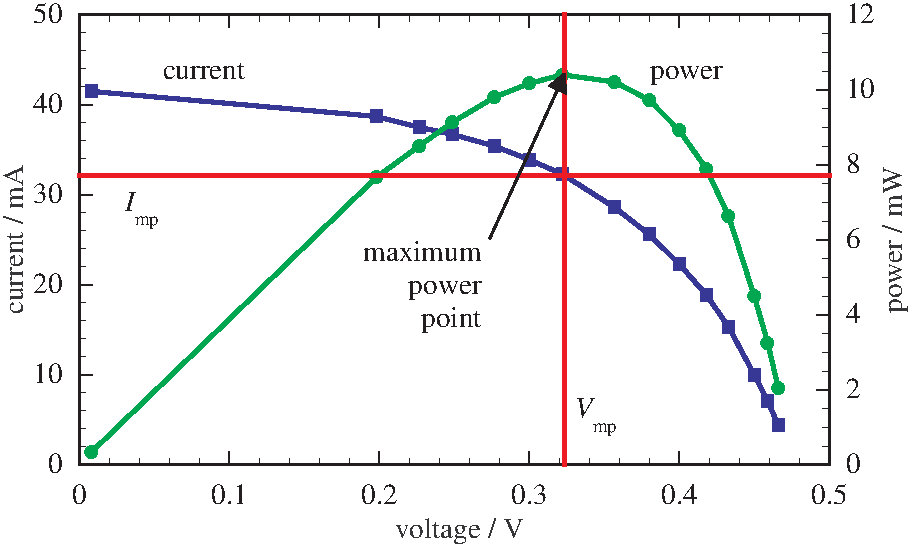
\includegraphics[scale=0.72]{solarcell}
\caption{Current and power as a function of voltage delivered by a single photovoltaic cell under illumination from a 150\,W metal halide floodlamp, showing the maximum power point.}
\label{solar cell fig}
\end{figure}

Figures and tables must have informative captions and be numbered as in Figure~\ref{solar cell fig}. Axes of graphs should have scales, titles and units, otherwise the plot is meaningless. All text must be legible, roughly the same size as the main text. Be warned that plots from Excel need extensive editing to bring them up to an acceptable standard. Oscilloscope screenshots can make good illustrations and are simple to capture on modern equipment.

Tables must have appropriate headings with units. Avoid lengthy tables: consider whether a graph would be clearer or the data would be better on a CD.

\subsection{References}

No project is done in isolation. A research project builds on the results of previous workers; a design-and-build project depends on the properties of the components available. You therefore draw on published documents during your project and must provide \emph{references} to these sources in your report. References are cited (a)~to give due credit to the originator and (b)~to guide a reader who wants more detailed information. You should give a reference wherever it is required for either of these purposes. Properly referenced material from many sources is a sign of a good project report. 
%This section explains how to present such references and how you will be penalised if you fail to do this. The mark for the report include an element for references to reflect their importance.

References must be cited with sequential numbers in square brackets where they are used in the text, not just listed at the end of the report. Typical usage is `Fitzmaurice and Hand \cite{gmf87} showed that\dots' or `The median is an appropriate estimator for this signal \cite{gmf87}'.

Avoid direct quotations from references in general; make it absolutely clear that the text is a quotation if this is unavoidable. An illustration, such as a diagram from a data sheet, is another type of quotation and must be referenced, typically in the figure caption. This is perfectly acceptable: do not waste time redrawing diagrams.

\subsubsection{Plagiarism}

If you copy from another person's work (project report, book, journal, web page or any other document) without acknowledging the source, you are guilty of \emph{plagiarism}. This is a disciplinary offence and the University has procedures for handling it. The failure to acknowledge a source is considered as plagiarism even if there was no deliberate intention to cheat. 

Avoid any risk of plagiarism by providing a reference for all sources that you use. Read the advice offered by the University Library and consult your supervisor if you are in any doubt. The University's \emph{Plagiarism Statement} is reproduced in Appendix \ref{plagiarism sect}.

\subsubsection{List of references}

All reports must have a section entitled `References' after the main text but before any appendices. This comprises a list of references, numbered to match the citations in the text. Each reference requires the following information and the cited references provide examples.
\begin{itemize}
\item
\textbf{Journal paper}: 
author(s), title of paper, name of journal, volume number, first page, last page and year \cite{gmf87}. 
Many journals now use article numbers instead of page numbers.
\item
\textbf{Book}: 
author(s), title, edition, publisher and year of publication \cite{jve05}.
Include the number of the chapter or page(s) if you refer to only a small part of the book.
\item
\textbf{Data sheet}: 
company, title, edition and date \cite{s08qg}. 
Application notes, technical reports and similar documents should be cited in the same way.
\item
\textbf{Web page}: 
author(s) or organisation, title, full URL and date of viewing \cite{mac09}. See below.
\end{itemize}
%The general rule is that 
The reader must be able to find the document without searching for further information.

\subsubsection{References from the Web}

The World Wide Web is a wonderful resource because it is so easy to search. It is therefore tempting to use web pages as references. \emph{Proceed with caution} because the accuracy of many web sites cannot be verified. This is particularly true for anonymous sites such as Wikipedia. Use them only as a starting point: good pages provide references to more authoritative sources.

Reports whose references are all or mainly from the web, especially from anonymous sites, will be penalised.


\section{Discussion}

The discussion is your opportunity to impress an expert with your depth of understanding. Don't worry so much about the non-expert reader -- she or he can skip to the Conclusions.

For a research project this section should provide a logical argument leading from the experimental observations to the final conclusions. Evaluate your results thoroughly and gain every possible piece of understanding from them. Compare the results in detail to other work in the field. This should be a \emph{critical} comparison so don't just say that your results are different from previous work; explain \emph{why}. Never say `The results were as expected' unless you have already described exactly what was expected!

The main purpose of the Discussion in a design-and-build project is to assess the performance of your product against the specification, showing its strengths and weaknesses.


\section{Conclusions}

Every report must have conclusions, built on the discussion. This section includes a summary of the main achievements of the work but is more than that. The noun `conclusion' can be defined as `a judgement or decision reached by reasoning' \cite{oupconc} so you should highlight what has been learnt as a result of your project. What is the big picture that the reader should take away? 

The Conclusions should include an assessment of the outcome against the original aims of the project. If you were unable to fulfil some aims, explain why. It is also useful to review the project plan (which should be included with the report). Did some tasks prove to be unexpectedly difficult, for instance?

\subsection{Suggestions for further work}

Almost every project leaves you with ideas for the future. Research typically answers some questions while opening new ones; by the end of a design-and-build project you may have thought of a superior approach. Examiners are impressed by intelligent suggestions for further work because they show that you really understand the project. It is often a sign of strength to identify the weak points and suggest solutions for them.


\clearpage % start appendices on a new page
\begin{thebibliography}{9}
%\addcontentsline{toc}{section}{References}
\bibitem{jve05}
Joan van Emden,
\textit{Writing for Engineers},
3rd Edition,
Palgrave Macmillan 
(2005).

\bibitem{mkm06}
Marun K. Mitra,
\textit{Effective Technical Communication: A Guide for Scientists and Engineers},
Oxford
(2006).

\bibitem{dfb09}
David F. Beer and David McMurrey,
\textit{A Guide to Writing as an Engineer},
3rd Edition,
Wiley
(2009).

\bibitem{tmy05}
Trevor M. Young,
\textit{Technical Writing A--Z: A Commonsense Guide to Engineering Reports and Theses},
American Society of Mechanical Engineers
(2005).

\bibitem{ronneberger2015unet}
O. Ronneberger, P. Fischer, and T. Brox,
\textit{U-Net: Convolutional networks for biomedical image segmentation},
in \textit{Proc. Medical Image Computing and Computer-Assisted Intervention (MICCAI)},
pp. 234--241,
2015.

\bibitem{isensee2021nnunet}
F. Isensee, P. F. Jaeger, S. A. A. Kohl, J. Petersen, and K. H. Maier-Hein,
\textit{nnU-Net: A self-configuring method for deep learning-based biomedical image segmentation},
Nature Methods,
\textbf{18},
203--211
(2021).

\bibitem{staal2004drive}
J. Staal, M. D. Abramoff, M. Niemeijer, M. A. Viergever, and B. van Ginneken,
\textit{Ridge-based vessel segmentation in color images of the retina},
IEEE Transactions on Medical Imaging,
\textbf{23}(4),
501--509
(2004).

\bibitem{hoover2000locating}
A. Hoover, V. Kouznetsova, and M. Goldbaum,
\textit{Locating blood vessels in retinal images by piecewise threshold probing of a matched filter response},
IEEE Transactions on Medical Imaging,
\textbf{19}(3),
203--210
(2000).

\bibitem{fraz2012ensemble}
M. M. Fraz, A. R. Rudnicka, C. G. Owen, and S. A. Barman,
\textit{An ensemble classification-based approach applied to retinal blood vessel segmentation},
IEEE Transactions on Biomedical Engineering,
\textbf{59}(9),
2538--2548
(2012).

\bibitem{budai2013robust}
A. Budai, R. Bock, A. Maier, J. Hornegger, and G. Michelson,
\textit{Robust vessel segmentation in fundus images},
International Journal of Biomedical Imaging,
\textbf{2013},
154860
(2013).

\bibitem{luo2025panet}
X. Luo, L. Peng, Z. Ke, J. Lin, and Z. Yu,
\textit{PA-Net: A hybrid architecture for retinal vessel segmentation},
Pattern Recognition,
\textbf{161},
111254
(2025).

\bibitem{lee2015dsn}
C.-Y. Lee, S. Xie, P. Gallagher, Z. Zhang, and Z. Tu,
\textit{Deeply-supervised nets},
in \textit{Proc. Artificial Intelligence and Statistics (AISTATS)},
pp. 562--570,
2015.

\bibitem{zhu2021deformabledetr}
X. Zhu, W. Su, L. Lu, B. Li, X. Wang, and J. Dai,
\textit{Deformable DETR: Deformable transformers for end-to-end object detection},
in \textit{Proc. International Conference on Learning Representations (ICLR)},
2021.

\bibitem{zhu2019dcnv2}
X. Zhu, H. Hu, S. Lin, and J. Dai,
\textit{Deformable ConvNets v2: More deformable, better results},
in \textit{Proc. IEEE/CVF Conference on Computer Vision and Pattern Recognition (CVPR)},
pp. 9308--9316,
2019.

\bibitem{hou2021coordatt}
Q. Hou, D. Zhou, and J. Feng,
\textit{Coordinate attention for efficient mobile network design},
in \textit{Proc. IEEE/CVF Conference on Computer Vision and Pattern Recognition (CVPR)},
pp. 13713--13722,
2021.

\bibitem{qi2023dsc}
J. Qi, Y. He, Y. Liu, and X. Xu,
\textit{Dynamic snake convolution based on topological geometric constraints for tubular structure segmentation},
in \textit{Proc. IEEE/CVF International Conference on Computer Vision (ICCV)},
pp. 6070--6079,
2023.

\bibitem{gmf87}
G M Fitzmaurice and D J Hand, 
\textit{A comparison of two average conditional error estimators}, 
Pattern Recognition Letters, 
\textbf{6}, 
221--228 
(1987).

\bibitem{s08qg}
Freescale Semiconductor,
\textit{Datasheet for MC9S08QG microcontroller},
revision 4
(2008).

\bibitem{mac09}
Morgan Advanced Ceramics, 
\textit{Advanced Ceramics: Silicon Nitride}, \texttt{www.morgantechnicalceramics.com} 
(viewed 2009 May 13).

\bibitem{oupconc}
Oxford University Press, 
\textit{AskOxford},
\texttt{www.askoxford.com/?view=uk}
(viewed 2009 May 13).

`Conclusion' is defined as (1)~an end or finish, (2)~the summing-up of an argument or text, (3)~a judgement or decision reached by reasoning or (4)~the settling of a treaty or agreement.
\end{thebibliography}

\clearpage % start appendices on a new page
\appendix

\section{Appendices}

Use appendices for supporting material which is relevant but of a detailed nature. In this way the flow of ideas in the body of the report is not interrupted. Appendices are usually lettered rather than numbered to distinguish them. Several uses for appendices have been suggested already but bear in mind that a CD may be more appropriate for large tables of results, long programs and data sheets or other background information. Appendices are not included in the word count because the assessors are not obliged to read them. Do not put vital points here!

Include your project plan and interim reports as appendices on paper.

\section{University's Plagiarism Statement}
\label{plagiarism sect}

The University's degrees and other academic awards are given in recognition of a student's personal achievement. All work submitted by students for assessment is accepted on the understanding that it is the student's own effort. 

Plagiarism is defined as the submission or presentation of work, in any form, which is not one's own, without acknowledgement of the sources. Plagiarism includes inappropriate collaboration with others. Special cases of plagiarism can arise from a student using his or her own previous work (termed auto-plagiarism or self-plagiarism). Autoplagiarism includes using work that has already been submitted for assessment at this University or for any other academic award.

The incorporation of material without formal and proper acknowledgement (even with no deliberate intent to cheat) can constitute plagiarism. Work may be considered to be plagiarised if it consists of: 
\begin{itemize}
\item
a direct quotation; 
\item
a close paraphrase; 
\item
an unacknowledged summary of a source; 
\item
direct copying or transcription.
\end{itemize}
With regard to essays, reports and dissertations, the rule is: if information or ideas are obtained from any source, that source must be acknowledged according to the appropriate convention in that discipline; and any direct quotation must be placed in quotation marks and the source cited immediately. Any failure to acknowledge adequately or to cite properly other sources in submitted work is plagiarism. Under examination conditions, material learnt by rote or close paraphrase will be expected to follow the usual rules of reference citation otherwise it will be considered as plagiarism. Departments should provide guidance on other appropriate use of references in examination conditions. 

Plagiarism is considered to be an act of fraudulence and an offence against University discipline. Alleged plagiarism, at whatever stage of a student's studies, whether before or after graduation, will be investigated and dealt with appropriately by the University.

The University reserves the right to use plagiarism detection systems, which may be externally based, in the interests of improving academic standards when assessing student work.

\end{document}
